%%%%%%%%%%%%%%%%%%%%%%%%%%%%%%%%%%%%%%%%%%%%%%%%%%%%%%%%%%%%%%%%%%%%%%%%%%%%%%%%
\chapter{Разработка модуля для Clang}
%%%%%%%%%%%%%%%%%%%%%%%%%%%%%%%%%%%%%%%%%%%%%%%%%%%%%%%%%%%%%%%%%%%%%%%%%%%%%%%%

%%%%%%%%%%%%%%%%%%%%%%%%%%%%%%%%%%%%%%%%%%%%%%%%%%%%%%%%%%%%%%%%%%%%%%%%%%%%%%%%
\section{Список доступных проверок}
%%%%%%%%%%%%%%%%%%%%%%%%%%%%%%%%%%%%%%%%%%%%%%%%%%%%%%%%%%%%%%%%%%%%%%%%%%%%%%%%

%%%%%%%%%%%%%%%%%%%%%%%%%%%%%%%%%%%%%%%%%%%%%%%%%%%%%%%%%%%%%%%%%%%%%%%%%%%%%%%%
\subsection{Одинковые условия}
\label{sec:eqBin}
Часто во время написания кода программист может допустить опечатку и не заметить следующюю
логическую ошибку: в исходном коде имеется оператор сравнения,логический или побитовый в левой 
и правой части которого находятся одинаковые выражения. 

Рассмотрим пример:
\begin{lstlisting}
if (pos.x==0 && pos.x==0)
\end{lstlisting}

В данном случае слева и справа от оператора \&\& расположены одинаковые выражения pos.x==0,
что скорее всего свидетельствует о наличие ошибки, допущенной из-за невнимательности. Корректный код,
не вызывающий ошибок должен выглядеть так:
\begin{lstlisting}
if (pos.x==0 && pos.y==0)
\end{lstlisting}

%%%%%%%%%%%%%%%%%%%%%%%%%%%%%%%%%%%%%%%%%%%%%%%%%%%%%%%%%%%%%%%%%%%%%%%%%%%%%%%%
\subsection{Одинаковые ветки if-else}
\label{sec:eqStmt}
Данное предупреждение выдается на фрагмент кода, в котором полностью совпадают истинная и ложная ветка 
оператора "if". Такую опечатку нетрудно допустить при копировании кода.

Пример:
\begin{lstlisting}
if (isCorrect())
	flags |= CORRECT;
else
	flags |= CORRECT;
\end{lstlisting}

Скорее всего это неверный код и его стоит пересмотреть.

%%%%%%%%%%%%%%%%%%%%%%%%%%%%%%%%%%%%%%%%%%%%%%%%%%%%%%%%%%%%%%%%%%%%%%%%%%%%%%%%
\subsection{Одинаковые уловия в if-else-if}
\label{sec:eqCond}
Данная ошибка часто появляется в результате множественного копирования исходного кода после чего 
некоторые условия не были исправленны и остались прежними.

Рассмотрим пример:
\begin{lstlisting}
if (x==1)
	Func1();
else if (x==2)
	Func2();
else if (x==1)
	Func3();
\end{lstlisting}

В приведенном выше коде функция "Func3()" никогда не будет вызванна так как условия "x==1" уже
проверялось. Корректный код должен быть:
\begin{lstlisting}
if (x==1)
	Func1();
else if (x==2)
	Func2();
else if (x==3)
	Func3();
\end{lstlisting}

%%%%%%%%%%%%%%%%%%%%%%%%%%%%%%%%%%%%%%%%%%%%%%%%%%%%%%%%%%%%%%%%%%%%%%%%%%%%%%%%
\subsection{Ошибки использования функции memset}
\label{sec:memset}
Для обнуления области памяти часто используется функция memset. Но из-за невнимательности программист может 
перепутать местами второй и третий аргумент в результате чего не происходит обнуления:
\begin{lstlisting}
memset(buf,sizeof(buf),0)
\end{lstlisting}
Помимо приведенной выше ошибки, часто неопытные специалисты не знают, что третьим аргументом 
функции memset принимается значение в байтах.

Рассмотрим пример:
\begin{lstlisting}
int arr[10];
memset(arr, 0, 10);
\end{lstlisting}
В данном примере только первые 10 байт массива arr будут заполнены 0. Анализатор выдает предупреждения, 
только в том случае, когда третий аргумент не является кратным размеру типа первого аргумента. 
Если первым аргументом передается указатель, имеющий тип не char,short,int или long, а третьим константа, то
выдается предупреждение, что не стоит использовать константу.

%%%%%%%%%%%%%%%%%%%%%%%%%%%%%%%%%%%%%%%%%%%%%%%%%%%%%%%%%%%%%%%%%%%%%%%%%%%%%%%%
\subsection{Неверный размер для выделения памяти под строку}
\label{sec:allocStr}
Часто многие начинающие и даже опытные программист забывают что в C/C++ строки должны заканчиваться
терминальным символом '\\0'. В результате появляется ошибка недостаточного выделения памяти под строку.

Пример:
\begin{lstlisting}
char * str = (char)malloc(strlen(name));
strcpy(str, name);
\end{lstlisting}

В результате выполнения приведенного кода будет выход за предел выделенной памяти. Поэтому необходимо
использовать следующий код:
\begin{lstlisting}
char * str = (char)malloc(strlen(name)+1);
strcpy(str, name);
\end{lstlisting}

Ошибка так же находится в случае, если для выделения памяти используется оператор \textbf{new}

%%%%%%%%%%%%%%%%%%%%%%%%%%%%%%%%%%%%%%%%%%%%%%%%%%%%%%%%%%%%%%%%%%%%%%%%%%%%%%%%
\subsection{Опечатка при использовании strlen}
\label{sec:strlen}
Как уже описывалось ранее, для хранения строк в С/С++ необходимо не забыть про наличие терминального
символа '\\0'. Однако иногда из-за невнимательности можно поставить неправильно закрывающуюся скобку:
\begin{lstlisting}
char * str = (char)malloc(strlen(name+1));
strcpy(str, name);
\end{lstlisting}

В результате выделяется на двай байта меньше памяти, чем необходимо. 

Предупреждение о потенциальной ошибке выдастся только в случае, если в качестве аргумента
strlen является выражение сложения, правой частью которого является литера \textbf{1}.

%%%%%%%%%%%%%%%%%%%%%%%%%%%%%%%%%%%%%%%%%%%%%%%%%%%%%%%%%%%%%%%%%%%%%%%%%%%%%%%%
\subsection{Потенциальная ошибка при использовании strcmp в условии}
\label{sec:strcmp}
Часто по незнанию начинающие специалисты не знают как работают функции "strcmp" и "strncmp".
Данные функции используются для сравнения двух строк и возвращают 0, если строки совпадают.
Рассмотрим пример:
\begin{lstlisting}
if (strcmp(str1, str2))
\end{lstlisting}
 
Условие в операторе if выполняется только в том случае, когда строки не совпадают. Однако человек,
редко использующий данные функции может подумать, что условие истинно когда строки совпадают.
Хотя приведенный код не содержит ошибку, лучше переписать его следующим образом:
\begin{lstlisting}
if (strcmp(str1, str2) != 0)
\end{lstlisting}

%%%%%%%%%%%%%%%%%%%%%%%%%%%%%%%%%%%%%%%%%%%%%%%%%%%%%%%%%%%%%%%%%%%%%%%%%%%%%%%%
\subsection{Одинаковые аргументы функций strcmp,strncmp,memmove,memcpy,strstr}
\label{sec:eqArgs}
Часто в программе происходит вызов функции, в которую передается два одинаковых аргумента и для
многих функций такая ситуация является нормальной. Однако для таких функций как strcmp,strncmp,memmove,memcpy,strstr
такая ситуация является подозрительной.

%%%%%%%%%%%%%%%%%%%%%%%%%%%%%%%%%%%%%%%%%%%%%%%%%%%%%%%%%%%%%%%%%%%%%%%%%%%%%%%%
\subsection{Выражение внутри sizeof}
\label{sec:sizeof}
Выражения написанные внутри оператора sizeof не выполняются, поэтому такой фрагмент кода является подозрительным.

Рассмотрим пример:
\begin{lstlisting}
int i=0;
size_t normalSize = sizeof(i++);
size_t doubleSize = sizeof(i *2);
\end{lstlisting}

В результате выполнения переменная i не увеличится и останется равной 0, а переменная doubleSize
будет равна переменной normalSize, хотя скорее всего в данном случае программист надеялся получить
значение в два раза больше. 

%%%%%%%%%%%%%%%%%%%%%%%%%%%%%%%%%%%%%%%%%%%%%%%%%%%%%%%%%%%%%%%%%%%%%%%%%%%%%%%%
\subsection{Перемножение операторов sizeof}
\label{sec:sizeofMul}
Исходный код, в котором происходит перемножение двух операторов sizeof(), практически всегда
свидетельствует о наличии ошибки.

Рассмотрим пример:
\begin{lstlisting}
TCHAR buf[256];
DWORD count = sizeof(buf)*sizeof(TCHAR);
\end{lstlisting}

В данном коде тип TCHAR определяется во время компиляции и в зависимости от настроек
может иметь размер один и более байт. В результате при размере THCAR больше одного байта,
количество элементов буффера будет неверным. 

Для корректного определения количество элементов необходимо использовать следующий код:
\begin{lstlisting}
TCHAR buf[256];
DWORD count = sizeof(buf)/sizeof(TCHAR);
\end{lstlisting}

%%%%%%%%%%%%%%%%%%%%%%%%%%%%%%%%%%%%%%%%%%%%%%%%%%%%%%%%%%%%%%%%%%%%%%%%%%%%%%%%
\subsection{Выделение памяти для одного простого типа с инициализацией}
\label{sec:new}
Если в коде происходит динамическое создание одного единственного целочисленного объекта с
инициализацией, то скорее всего произошла опечатка и программист хотел использовать
квадратные скобки вместо круглых.

Пример:
\begin{lstlisting}
int *arr = new int(N);
\end{lstlisting}

Предупреждение появляется только при попытке создания объекта с типом char, short, int или long.

%%%%%%%%%%%%%%%%%%%%%%%%%%%%%%%%%%%%%%%%%%%%%%%%%%%%%%%%%%%%%%%%%%%%%%%%%%%%%%%%
\subsection{Сравнение указателя и 0}
\label{sec:ptrCmp}
Анализатор выдает предупреждение при нахождении сравнения указателя и литеры 0 с ипользованием 
оператора \textbf{<}.

Пример кода:
\begin{lstlisting}
class ResourceManager
{
public:
	SomeObj* Find(const char * filename);
	void LoadResource(const char * filename);
	...
} resources;
...
if (resources.Find("foo") < 0)
	resources.LoadResource("foo");
\end{lstlisting}
  
Приведенный выше код мог легко появится в процессе рефакторинга если раньше был следующий код: 
\begin{lstlisting}
class ResourceManager
{
public:
	int Find(const char * filename);
	SomeObj* Get(int index);
	void LoadResource(const char * filename);
	...
} resources;
...
if (resources.Find("foo") < 0)
	resources.LoadResource("foo");
\end{lstlisting}
Метод "Find" изначально возвращала индекс, по которому можно было получить ресурс, если же 
ресурс не был найден, возвращалось -1. Но после рефакторинга метод "Find" стал возвращать указатель на 
ресурс или 0, в результате метод LoadResource никогда не будет вызван.

%%%%%%%%%%%%%%%%%%%%%%%%%%%%%%%%%%%%%%%%%%%%%%%%%%%%%%%%%%%%%%%%%%%%%%%%%%%%%%%%
\section{Диаграмма классов}
%%%%%%%%%%%%%%%%%%%%%%%%%%%%%%%%%%%%%%%%%%%%%%%%%%%%%%%%%%%%%%%%%%%%%%%%%%%%%%%%
\begin{figure}[H]
\centering
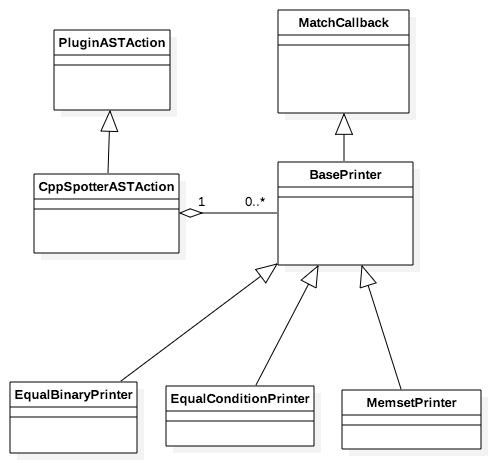
\includegraphics[width=\textwidth]{UML}
\caption{UML диаграмма классов}%
\label{fig:UML}
\end{figure}

Тут стоит описать как относятся классы друг к другу?

%%%%%%%%%%%%%%%%%%%%%%%%%%%%%%%%%%%%%%%%%%%%%%%%%%%%%%%%%%%%%%%%%%%%%%%%%%%%%%%%
\section{Динамическое подключение проверок}
%%%%%%%%%%%%%%%%%%%%%%%%%%%%%%%%%%%%%%%%%%%%%%%%%%%%%%%%%%%%%%%%%%%%%%%%%%%%%%%%
Невсегда удобно использовать все доступные проверки. В случае если какая-то проверка на ошибки
выдает слишком много ложных предупреждений, ее лучше отключить и сосредоточиться на более важных
ошибках. 

Для включения нужных проверок необходимо использовать следующие флаги:
\begin{itemize}
	\item \textbf{-eqBin}	Одинаковые условия, см. \ref{sec:eqBin}
	\item \textbf{-eqStmt}	Одинаковые ветки if-else, см. \ref{sec:eqStmt}
	\item \textbf{-eqCond}	Одинаковые условия в if-else-if, см. \ref{sec:eqCond}
	\item \textbf{-memset}	Неверное использование memset, см. \ref{sec:memset}
	\item \textbf{-allocStr}	Неверный размер для выделения памяти под строку, см. \ref{sec:allocStr}
	\item \textbf{-strlen}	Опечатка при использовании strlen, см. \ref{sec:strlen}
	\item \textbf{-strcmp}	Потенциальная ошибка strcmp, см. \ref{sec:strcmp}
	\item \textbf{-eqArgs}	Одинаковые аргументы функций, см. \ref{sec:eqArgs}
	\item \textbf{-sizeof}	Выражение внутри sizeof, см. \ref{sec:sizeof}
	\item \textbf{-sizeofMul}	Перемножение операторов sizeof, см. \ref{sec:sizeofMul}
	\item \textbf{-new}		Выделение памяти для одного простого типа, см. \ref{sec:new}
	\item \textbf{-ptrCmp}	Сравнение указателя и 0, см. \ref{sec:ptrCmp}
	\item \textbf{-all}		Включение всех вышеперечисленных проверок
\end{itemize}

Для передачи каждого флага в плагин необходимо использовать следующий формат:
\begin{lstlisting}
-plugin-arg-<имя плагина> <флаг> 
\end{lstlisting}
Где <имя плагина> соответствует имени плагина, которое задается 
в исходном коде при регистрации плагина, а <флаг> соответсвует флагу, который получет плагин.
Так для того, чтобы включить проверки одинаковых условий (\ref{sec:eqBin}) и сравнения указателя с 0 (\ref{sec:ptrCmp}),
нужно передать Clang такие ключи:
\begin{lstlisting}
-plugin-arg-CppSpotter -eqBin \ 
-plugin-arg-CppSpotter -ptrCmp  
\end{lstlisting}


%%%%%%%%%%%%%%%%%%%%%%%%%%%%%%%%%%%%%%%%%%%%%%%%%%%%%%%%%%%%%%%%%%%%%%%%%%%%%%%%
\section{Добавление новых проверок}
%%%%%%%%%%%%%%%%%%%%%%%%%%%%%%%%%%%%%%%%%%%%%%%%%%%%%%%%%%%%%%%%%%%%%%%%%%%%%%%%
Добавление новой проверки происходит в три этапа:
\begin{enumerate}
	\item Создание класса обработчика. Данный класс необходим для обработки подозрительных мест
в исходном коде и в случае нахождения ошибки отвечает за отображение предупреждения. Созданный класс
должен наследоваться от класса BasePrinter и переопределять функцию
\begin{lstlisting}
void addToFinder(ast_matchers::MatchFinder * finder)
\end{lstlisting} 
Эта функция отвечает за регистрацию созданного обработчика.
	\item Создание AST Matcher для выявления узлов абстрактного синтаксического дерева, потенциально 
содержащих ошибки. Созданный AST Matcher используется при регистрации обработчика в функции 
\textbf{addToFinder}.
	\item Последним этапом является добавление нового флага для созданной проверки в функции 
\textbf{ParseArgs}. Если пользователь передал флаг на включение новой проверки, необходимо
добавить данную проверку в список используемых проверок с помощью функции \textbf{addPrinter}.
\end{enumerate}
